\documentclass[12pt]{article}
\usepackage[T1]{fontenc} 
\usepackage[portuguese]{babel}
\usepackage{hyphenat}
% use se você precisar forçar a separação de sílabas em quebra de linha
\hyphenation{mate-mática recu-perar}
\usepackage{graphicx}
\graphicspath{images/}
\usepackage{csquotes}
\usepackage{subfiles}
\usepackage{amsmath}
\usepackage{csvsimple} 
\usepackage{geometry}
\geometry{
    a4paper,
    left=3cm,
    top = 3cm,
    right=2cm,
    bottom=2cm
}
\setlength{\parindent}{4em}
%\setlength{\parskip}{1em}
\renewcommand{\baselinestretch}{1.5}

\usepackage[dvipsnames]{xcolor}
\definecolor{alert}{RGB}{201, 58, 128}
\setlength {\marginparwidth }{2cm} 
\usepackage[colorinlistoftodos]{todonotes}
\usepackage{comment}
\usepackage{subcaption}
\DeclareUnicodeCharacter{0301}{*************************************}
\usepackage{enumitem}

\title{TÍTULO}
\author{autor}

\begin{document}

% CAPA
\thispagestyle{empty}

    
    \begin{flushright}
        \begin{huge}
            \textbf{RELATÓRIO}\\[3,5cm]
        \end{huge}
%% CSS: Podemos usar um título mais genérico agora e depois discutir um definitivo
{\bf \LARGE  CLASSIFICAÇÃO DE GLAUCOMA EM IMAGENS DE FUNDO DE OLHO COM APRENDIZAGEM PROFUNDA}

\bigskip
        
        Leandro Zangirolami Trovões (Orientando)\\
        Carlos da Silva dos Santos (Orientador)\\
        Universidade Federal do ABC\\[5,5cm]
    \end{flushright}

    \vfill
    
    \begin{center}
        Santo André,\\
        Setembro de 2024
    \end{center}
    
    \newpage
\bigskip

\begin{center}
\noindent{\bf \Large Resumo}
\end{center}

\begin{quote}
[Contexto, visão geral do método, etc]
\end{quote}

\begin{center}
Santo André, setembro de 2024
\end{center}

\newpage
\bigskip

\section{Introdução}
\label{sec:introducao}

\begin{comment}
doença sem cura, caracterizada pelo aumento de pressão intra-ocular que causa dados ao nervo ótico.
buscar fonte, WHO Nao explica direito
\end{comment}

%% CSS: usar o ~ antes do \cite impede que o latex quebre linha entre 
%       o texto e a anotação
Principal causa de cegueira irreversível no mundo~\cite{steinmetz_causes_2021}, o glaucoma é uma doença sem cura, caracterizada pelo dano progressivo ao nervo ótico~\cite{who_2019}. Estima-se que, em 2020, 3,6 milhões de pessoas com 50 anos ou mais já tenham perdido a visão para o Glaucoma~\cite{steinmetz_causes_2021} e um estudo de 2014 ainda projeta que 111.8 milhões de pessoas sejam afetadas pela doença no ano de 2040.~\cite{tham_global_2014}.

Assintomática em seus estágios iniciais, conforme avança, a doença causa perda de visão periférica e, se não for tratada, pode levar a perda total da visão. O tratamento pode retardar ou prevenir a progressão, mas depende de um diagnóstico precoce, geralmente antes mesmo dos primeiros sintomas~\cite{who_2019}.

\begin{comment}
O tratamento consiste em reduzir a pressão intra-ocular e 

fatores de risco: idade, histórico familiar

OMS: General population screening for glaucoma is not currently
considered to be cost-effective in most settings (63). Therefore,
routine eye examinations are recommended for high-risk individuals
as early detection is essential for the protection of visual function. 
\end{comment}

Uma das formas de identificar a presença de glaucoma é por meio da fundoscopia ou exame de fundo de olho, no qual é possível observar alterações características, muitas vezes antes mesmo que a perda de visão se torne detectável~\cite{weinreb_2004}. Um exemplo de imagem obtida nesse exame é apresentado na Figura~\ref{fig:fundus}.

A principal característica observada ao analisar o fundo de olho é o tamanho da escavação em relação ao tamanho do disco ótico do paciente, ambos destacados na Figura~\ref{fig:disk}. O disco ótico é a região em que as células da retina se convergem para formar o nervo ótico. Essa convergência forma uma depressão ao centro do disco, chamada de escavação (em inglês conhecido como \emph{optic cup}). O anel neurorretiniano é a região que envolve a escavação. A razão entre o tamanho do disco e da escavação é conhecida como razão disco-copo (em inglês \emph{cup-to-disk ratio}) e seu valor acima do normal é um indicativo do dano causado pela doença ~\cite{weinreb_2004}. % posso também citar weinreb_2016 para essa última afirmação

\begin{figure}[htb]
 \centering
 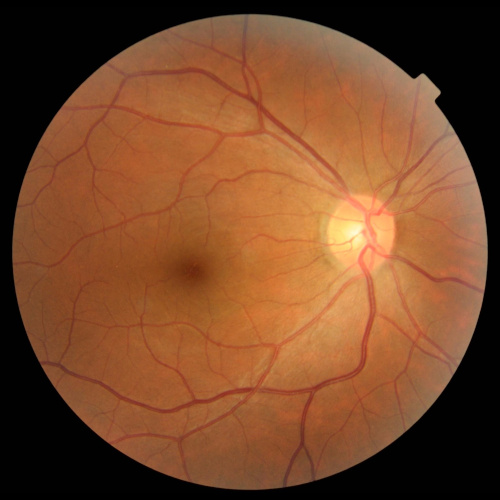
\includegraphics[width=0.3\textwidth]{images/TRAIN000004_cut.JPG}
 \caption{Imagem de fundo de olho. Obtida do banco de dados JustRAIGS.}
 \label{fig:fundus}
\end{figure}

\begin{comment}
Dentre as características observadas estão: 1, 2, 3, 4 e 5. cite{"Five rules to evaluate the optic disc and retinal nerve fiber layer for glaucoma"}

A capacidade da inteligência artificial em --- atrai seu uso na medicina. cite{alguem}

uso de IA com imagens médicas aumentou\\


fazer a avaliação manual gera divergência entre médicos, falta de padronização -> podemos fazer de forma automática
\end{comment}

\begin{comment}
da pra falar que médicas acreditam no potencial da IA
tem essa pesquisa aqui mas me parece muito restrita: só australia e nova zelancia e só com  trainees
...médicos acreditam que IA vai melhorar o trabalho deles... \cite{scheetz_survey_2021}
\end{comment}


Recentemente, diversas técnicas de aprendizagem profunda vem sendo aplicadas no diagnóstico de doenças com base em imagens de fundo de olho, inclusive para o glaucoma~\cite{li_review_2021}. Para possibilitar o desenvolvimento desses modelos, bancos de dados com imagens de fundo de olho classificadas por oftalmologistas foram criados e alguns deles disponibilizados publicamente, como o RIGA~\cite{riga}, ORIGA~\cite{origa}, RIM-ONE DL~\cite{RIMONEDL} e JustRAIGS~\cite{justraigs}. Um quadro resumo com alguns bandos de dados é apresentado na Tabela~\ref{tab:datasets}. 

\begin{figure}[htb]
 \centering
 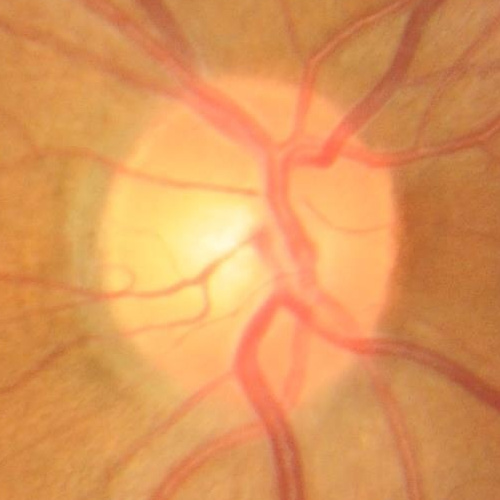
\includegraphics[width=0.3\textwidth]{images/disk.jpg}
 \caption{Disco ótico em destaque. Obtida do banco de dados JustRAIGS.}
 \label{fig:disk}
\end{figure}

% LZT: adicionar mais trabalhos aqui

Trabalhos anteriores conseguiram realizar a classificação de imagens entre glaucoma e não glaucoma utilizando diferentes técnicas. Noronha et al. (2014) utilizou cumulantes de alta ordem para identificar glaucoma em 272 imagens de fundo de olho obtidas por conta própria, obtendo acurácia de 84.72\% \cite{Noronha2014}. Chen et al. (2015) implementou uma rede neural convolucional, contendo seis camadas sendo quatro convolucionais e 2 totalmente conectadas, e a treinou em dois bancos de dados privados, obtendo de resultado os valores de área sobre curva (AUC) 0.831 e 0.887 \cite{chen2015glaucomadetection}. Um quadro resumo com estes e outros trabalhos é apresentado na Tabela~\ref{tab:trabalhos}.

% LZT: tentar explicar interpretabilidade e falar das features adicionais do JustRAIGS.
\begin{comment}
Uma das áreas para melhorias segundo Li, et al. \cite{li_review_2021} é questão à interpretabilidade dos resultados fornecidos pelos modelos de classificação, devido à característa de black-box inerente à modelos de aprendizagem profunda.
\end{comment}

O banco de dados JustRAIGS, além de incluir anotações entre a imagem ser referenciável para glaucoma ou não, também possui 10 anotações adicionais, para sinais observados pelos avaliadores, que justifiquem a escolha como referenciável para glaucoma, naquelas assim marcadas \cite{justraigs_article}.

O presente trabalho procura explorar o uso de redes neurais convolucionais no problema de classificação do glaucoma em imagens de fundo olho, além de investigar o uso das anotações adicionais presentes no JustRAIGS como forma de auxiliar na interpretabilidade dos resultados produzidos pelos modelos.

O restante do texto é organizado da seguinte maneira: em primeiro lugar, apresentamos os objetivos deste trabalho na Seção~\ref{sec:objetivo} e, em seguida, apresentamos na Seção~\ref{sec:schedule} o plano de trabalho proposto.

\begin{comment}
DESCONSIDERAR ESSE BLOCO

usando redes neurais\\
e até mesmo técnicas de processamento de sinais\cite{Noronha2014}

porem:
\begin{itemize}
 \item datasets limitados (agora temos um de 100k imagens) e alguns são privados
 \item falta de justificativa, blackbox ~\cite{li_review_2021} 7.2.5, usar features adicionais para explicar decisão
\end{itemize}

suposições que precisam ser sustentadas:\\
1- razão OD e OC é a melhor forma de identificar glaucoma\\
2- CNN é melhor de que calcular a razão ente OD e OC: [Chen, 2015] afirma mas não sustenta. Cita [3]\\

2) Diaz-Pinto, 2019: usando CNN não precisa fazer segmentação perfeita do OD e do OC
"Important limitations of the methods that are based on handcrafted characteristics (CDR, Area Cup/Disc ratio (ACDR), vessel kinks and ISNT rule) is the significant disagreement in estimating them even between expert human graders. For that reason, new algorithms have been focused on automatic feature extraction such as the data-driven methods [3] and convolutional neural networks (CNNs)."\\
Menciona alguns trabalhos que foram pela abordagem da segmentação e os resultados obtidos.

investigar:
Chen, 2015: 17 5 6 14, 2, 12, 13\\
Noronha, 2014: 9, 16, 17, 18

\end{comment}

\begin{table}[htb]
    \centering
    \begin{tabular}{|c|c|c|}
    \hline
    Nome & Nº de imagens & Ano de publicação \\
    \hline
    ORIGA & 650 & 2010 \\
    \hline
    DRISHTI-GS1 & 101 & 2015 \\
    \hline
    RIGA & 750 & 2018 \\
    \hline
    RIM-ONE DL & 485 & 2020 \\
    \hline
    REFUGE & 1200 & 2020 \\
    \hline
    JustRAIGS & 101.442 & 2024 \\
    \hline
    \end{tabular}
    \caption{Bancos de dados para avaliação de glaucoma}
    \label{tab:datasets}
\end{table}

% LZT: terminar tabela de trabalhos anteriores

\begin{table}[htb]
    \centering
    \begin{tabular}{|l|l|l|l|c|c|}
    \hline
    Autores          & Método          & Imagens & Banco        & ACC     & AUC   \\
    \hline
    Chen, 2015       & CNN própria     &         & ORIGA        & -       & 0.831 \\
    \hline
    Chen, 2015       & CNN própria     &         & ORIGA + SCES & -       & 0.887 \\
    \hline
    Noronha, 2014    & Cumulantes      & 272     &              & 0.847  &  -     \\
    \hline
    Diaz-Pinto, 2019 & Xception        &         & -            &        &        \\
    \hline
    \end{tabular}
    \caption{Trabalhos anteriores e resultados obtidos}
    \label{tab:trabalhos}
\end{table}

\bigskip

\section{Objetivos}
\label{sec:objetivo}

O objetivo geral deste trabalho é criar um modelo para classificação de glaucoma em imagens de fundo de olho que seja interpretável.

Os objetivos específicos são:
\begin{itemize}
 \item segmentação da região de interesse
 \item "comparar modelos quanto à interpretabilidade"
 \item determinar metodologia para comparar interpretabilidade
\end{itemize}


\begin{comment}
Resultados parciais

Para segmentar o disco ótico, a regiao de interesse a ser alimentada para o classificador, 
\end{comment}

\bigskip

\section{Plano de trabalho}
\label{sec:schedule}

O plano de trabalho


\begin{figure}[htb]
 \centering
 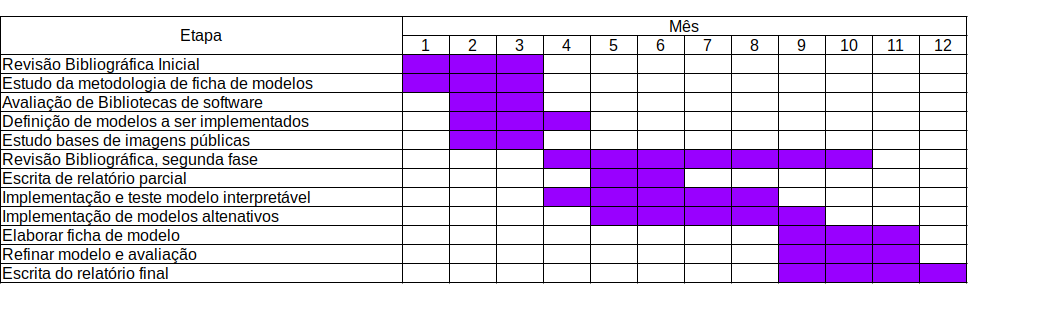
\includegraphics[width=1.0\textwidth]{images/crono2022}
 \caption{Cronograma de execução da proposta}
 \label{fig:crono}
\end{figure}

\bigskip

%% LZT: Como fazer para não incluir a lista completa de nomes? [SBB+21] ficou muito grande
\bibliographystyle{alpha}%{hapalike}
\bibliography{ref.bib}

\end{document}
